%\section{Blindenss}
%The majority of this analyses was designed with the data blinded in the
%relevant energy region.
%The data blinding was done primarily for a nucleon decay analysis~\citep{snop_nd}
%that was performed using the same dataset as this analyses, but was done
%for this analysis as well because both results were produced contemporaneously.
%
%%TODO check these numbers
%The scheme for blinding the data was to remove all events from the dataset that
%had an nhit between $30$ and $100$, this correspond to an approximate electron energy
%range of \numrange{4.0}{15.0}\,MeV.
%The analyses was designed primarily using simulation and a two-week open
%data period, on which no blindness restrictions were imposed.
%
%Part way through the analysis testing and design the data was partially un-blinded
%to allow for an initial look at the results.
%Blinded events that reconstructed energy between $4.5$\,MeV and $15.0$\,MeV
%were added into the dataset with all energy related information removed;
%each event was assigned the artificial energy of $10.0$\,MeV.
%With those data, plots of the distribution of event direction with respect to
%the sun were created and provided a check that the results were as expected.
%The energy cut used to select events for that plot was performed using
%un-calibrated energy, so it has little bearing on the results of the full
%analysis.

\section{Data Selection}
\label{sec:data_selection}
Events are included or removed from the dataset across three stages of selection.
First entire runs are either included or removed based upon whether they meet
certain criteria for data quality.
The events within selected runs are then rejected or approved by a set
of low-level cuts that attempt to remove events caused by instrumental
backgrounds and other sources of unwanted events.
Within events that pass the low-level cuts, hits can be rejected from consideration
if they're deemed unlikely to have originated from light within the detector.
Following that, analysis level cuts are applied to the reconstructed quantities
for each event.
The analysis cuts are designed to maximize the signal efficiency for dataset and minimize the
contamination from background sources.
Each of these steps are detailed below.

\subsection{Dataset}
\label{sec:dataset}
Data for this analysis was taken in SNO+'s initial water-phase data-taking
run.
Data taking started May 05 2017 (exactly 4 years after I
started my PhD) and ended December 25 the same year.
The data taking started with run $100000$ and concluded with run
$108416$, with each run being typically 1 hour long, though not
all runs are suitable for analysis.
In those runs approximately 185 days worth of useable data was taken,
with significant pauses for commissioning of ancillary detector components,
such as the water circulation systems, and for detector maintenance.
Data taking was restarted several months after the end of this dataset,
after the AV circulation pipes had been replaced to help reduce backgrounds
in the detector.

In the dataset there are a three different periods of data taking that are
given special treatment in this analysis
to be considered.
The first is the hot-spot period of runs;
an external water circulation pipe was observed to have
introduced backgrounds into the upper-portion of the detector, between the
PSUP and AV\@.
For data taken during this period of time analysis cuts were adjusted, as
will be discussed in Sec~\ref{sec:analysis_cuts}.
The elevated background levels lasted from run $100400$ to $102048$.

The other period of time that requires special treatment within the analysis
is due to significant adjustments to the detector trigger settings done approximately
half-way through the dataset.
So the dataset is split into a high and low trigger period, the high trigger
period being first.
The high trigger period started at run 100000 the low trigger period started
at run 104613.
The adjustment made was to raise the threshold on all channel threshold
by a single DAC count.
The result was a significant reduction in the observed dropout and noise rate
in the detector, which allowed for the trigger threshold to be pushed further
down, and an overall increase the detector's efficiency.

\begin{figure}[htbp]
    \centering
    \begin{subfigure}[b]{0.48\textwidth}
        \centering
        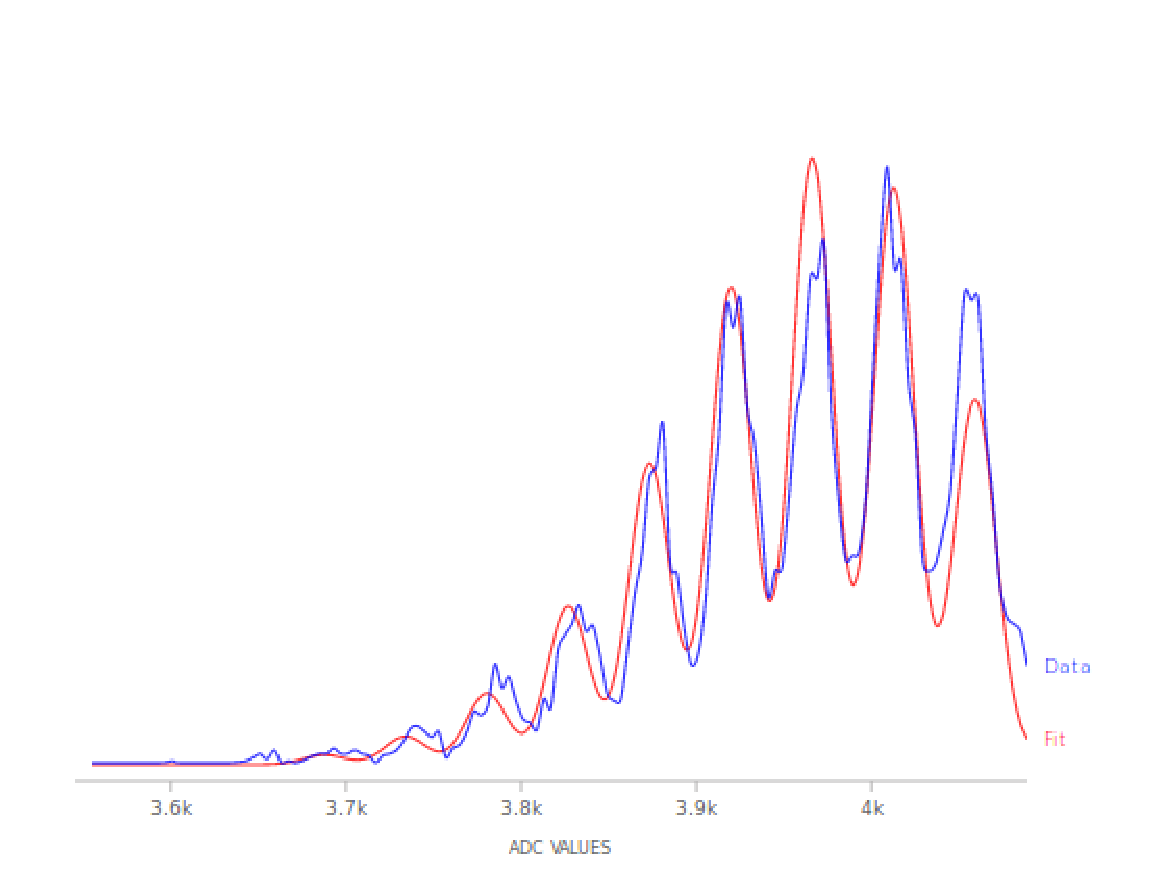
\includegraphics[width=\textwidth]{pre_trigger_dropout}
        \caption[]{}
    \end{subfigure}
    \hfill
    \begin{subfigure}[b]{0.48\textwidth}
        \centering
        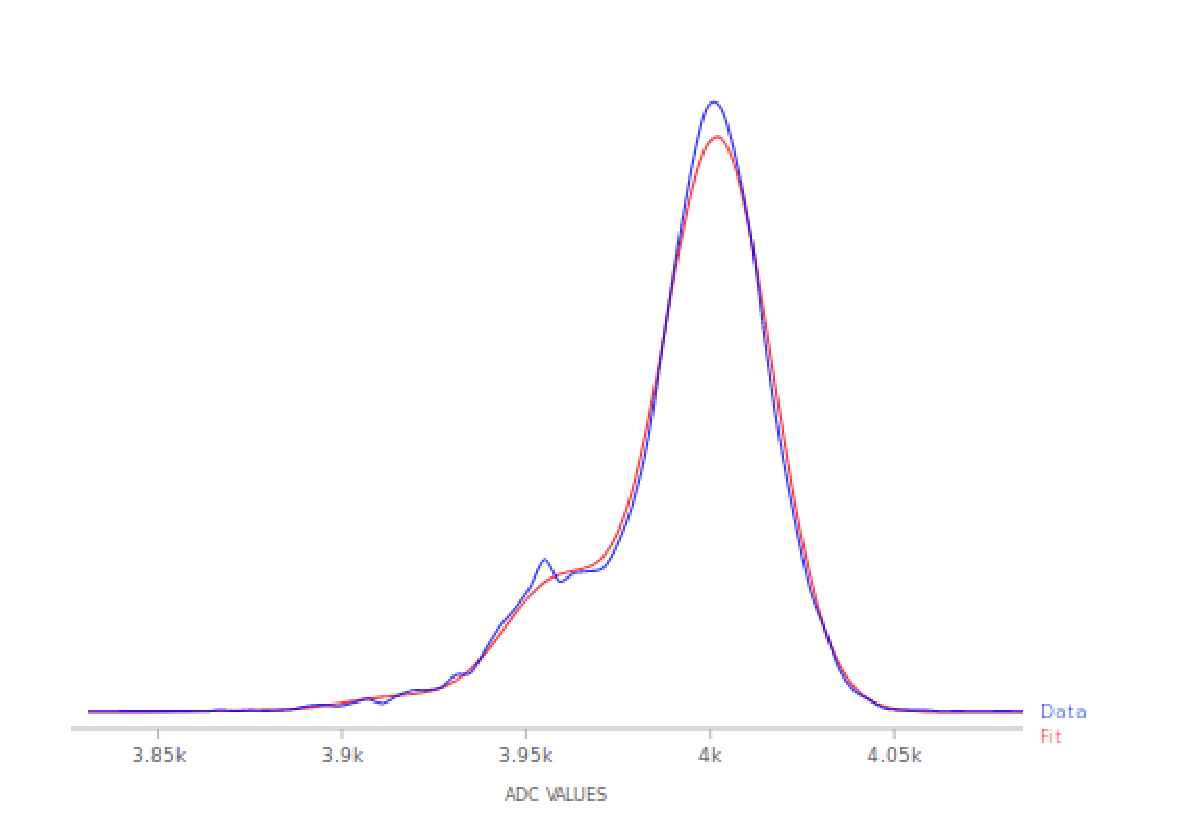
\includegraphics[width=\textwidth]{post_trigger_dropout}
        \caption[]{}
    \end{subfigure}

    \begin{subfigure}[b]{0.78\textwidth}
        \centering
        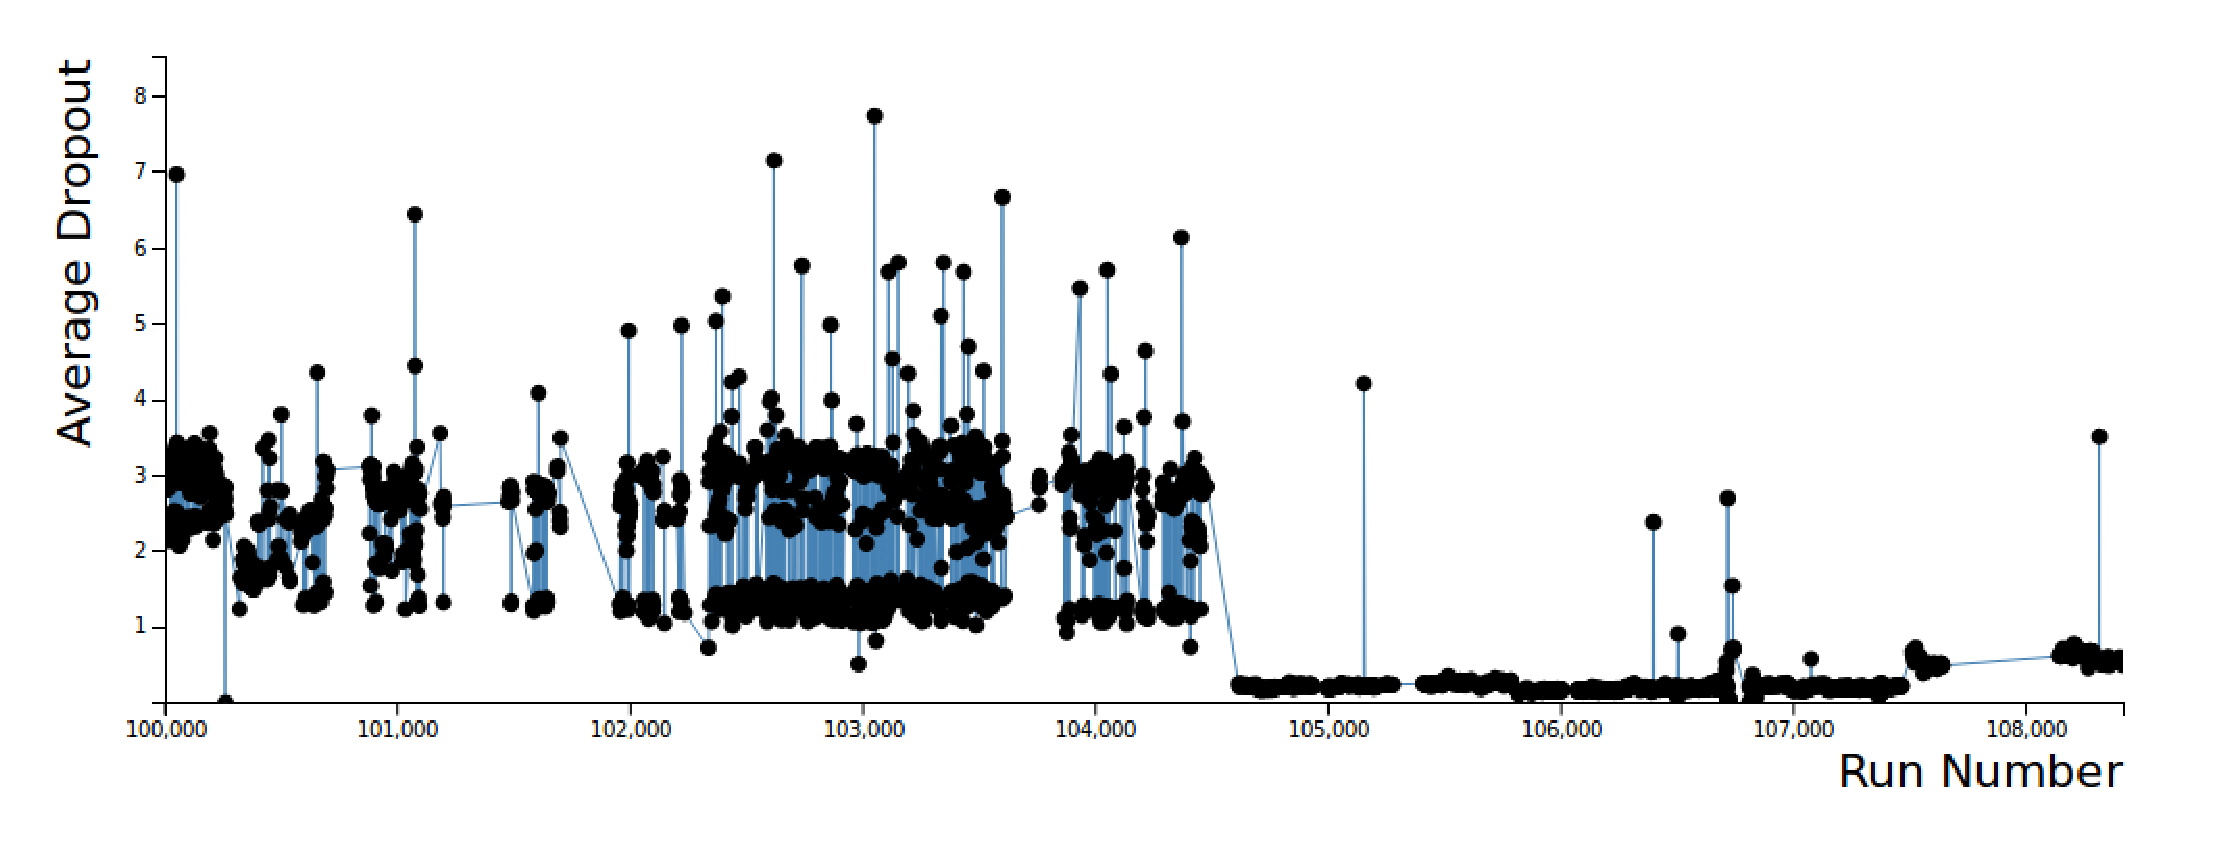
\includegraphics[width=\textwidth]{dropout_nd}
        \caption[]{}
    \end{subfigure}
    \caption[Dropout In Low and High Trigger Period]{
        N20 dropout in the high (a) and low (b) trigger period,
        and the average dropout measured across all runs in the
        dataset (c); the various ``jumps'' in the dropout are generally
        due to bad fits.}
    \label{fig:dataset_dropout}
\end{figure}
%
%It's not known why the adjustment to channel thresholds resulted in such a significant
%reduction in the rate.
%It may be the case that adjusting the threshold reduced the rate of dropout.
%Figure~\ref{fig:dataset_dropout} shows a dropout measurement before and after the trigger
%adjustment, which shows how significant the dropout rate reduction in the trigger
%system was.
%It's not known if the in dropout is a side-effect of the noise reduction in
%the system, or the cause of it.

\subsection{Run Selection}
\label{sec:run_selection}
Runs are rejected from the dataset if they fail to meet certain criteria
for data quality and detector stability.
It's first required that all meta-info about a run be created and stored
within the RAT Database successfully.
Those tables have information about the state of the hardware and DAQ, as
well as information about the run including the run type and length.
This information is necessary for assessing if the run is capable of being
used for a physics analysis.
It's further necessary that all meta-info be available so that the run
can be simulated.
It's very rare for the meta-info for a run not to be generated and stored
properly, so this check has a almost no effect on the dataset.

It's required that the run type of the run be ``PHYSICS'', this indicates
that the DAQ settings were not changed at any point in the run and no external
sources of events were present, and that the thresholds for triggering were set
at a level deemed sufficient for most physics analyses.
Following this checks are done
that require all electronics crates have high voltage on their PMTs throughout
the run.
It's also required that all channels that are at high voltage are capable of
reading out data, and that all crates are participating in the trigger sums.
A number of separate checks are performed to ensure that all necessary DAQ
processes were running well throughout the run, to ensure that the data taken
during the run was not interrupted by a lapse in the DAQ.\@

Beyond checks on the detector state and stability, a number of checks
are placed on the data taken within the run.
Most of these checks are placed on the rate of certain events within the detector.
It's required that the average ESUMH and N100L trigger rate be greater than 5Hz and
that the total trigger rate be less than 7kHz.
These checks ensure that the data taken during the run triggered the detector
at a rate consistent with standard running, during which the typical trigger
rate is near 1kHz.
Similarly it's required that fewer than 15\% of all events be retrigger events
(events that fall within 420\,ns of the previous event).
At a nominal rate of 1kHz it's very unlikely for two event to be within $420$\,ns
by chance, so a high rate of retrigger events might indicate a abnormally
high level of noise in the trigger system or light in the detector.
There are however events that can occur
in the detector, such as followers after a cosmic muon, that can produce
re-trigger events.
The cut threshold is designed to allow for retriggers from natural source but
still flag detector abnormalities.
These checks all ensure that the data in a run is likely to be useful for
a physics analysis, but are loose enough not to bias the dataset in a way that
might influence results.

\subsection{Livetime}
While most event selection removes individual events based upon whether they
pass or fail certain criteria, some cuts remove all events that occur for a
period of time before or after some criteria is met.
These cuts are said to introduce a deadtime into the dataset.
The most significant example of this is the muon follower data cleaning cut, which
cuts all events for 30\,seconds after every muon interaction in the detector.
The livetime for each run is then defined as
\begin{equation}
    t_{\mathrm{live}} = t_{run} - t_{\mathrm{dead}}\text{,}
\end{equation}
where $t_{run}$ is the time between the first and last valid event within a run
and $t_{\mathrm{dead}}$ is the sum of all deadtimes introduced into that run by cuts.
The livetime is used to calculate the total exposure represented by the dataset.
For simulated events many of the effects that necessitate deadtime are not simulated,
so no deadtimes are added into the simulated runs.
%Table XXX shows the sum of deadtimes across all runs within the dataset.
The livetime represented by the dataset is 120.2 days, after subtracting the
calculated deadtimes the effective livetime  114.7 days.

\subsection{Data Cleaning}
There are a number of instrumental effects that can cause an event
to be recorded by the detector, these events typically have some
sort of distinguishing feature or features that set them apart
from events that originate from particle interactions within the
detector.
A number of algorithms and cuts have been designed to identify and remove
these events from the dataset.
These algorithms are said to ``clean'' the data by removing events
of instrumental origin. These definition is extended to include removing
hits within an event that are likely of instrumental origin as well.

The primary type of instrumental event that must be removed is ``flashers'' and
``shark-fin'' events.
Both of these result from charge build-up on the PMT-base causing a
spark.
For a flasher event the light from the spark escapes through the PMT face
and illuminates the PMTs on the other side of the detector.
Flashers occur at a rate of a few per minute.
A shark-fin is similar but the spark is either small enough or located
in a position such that the light does not escape the PMT.\@
In both types of events the PMT in which the spark occurs with readout
a very high-charge hit, and the channels next to it on the FEC will
have low-charge hits from electronic pickup.
For shark-fin event no other channels will be hit, except possibly by an
accidental coincidence; for a flasher hit a number of hits will
occur from the light that escaped the PMT.\@
Since the number of PMT hits that occur in a flasher event can vary significantly,
anywhere between tens of hits and hundreds, they can reconstruct
to a wide range of energies and possibly contaminate a signal region.
Many data cleaning cuts are designed to ensure that all
flasher events are identified and removed from the dataset.

Within an event hits that are deemed unlikely to have come from a photon interacting with a PMT
are removed from the analysis through hit cleaning.
For this analysis the only sort of hits that were removed were those identified
as coming from cross-talk between adjacent channels in the detector.
Hits from cross-talk arise from stray capacitative coupling between adjacent, or nearby, channels
on a single daughter board.
Typically the noise from cross-talk will only be large enough to cause a hit
on adjacent channels if the original signal is relatively large.
The cross-talk hits will usually be especially low in charge because they're
the result of bi-polar noise, rather than a PMT signal, and the cross-talk
hit will always show up after the original hit.
These criteria are codified as a cut on any hits that show up within
 six channels from a hit that has a pedestal subtracted QHS greater
than 50\,ADC counts. Of those hits if it has a pedestal subtracted QHS between
$10$ and $-30$ and are between 9 and 25\,ns after the high charge hit,
then the hit is flagged a cross-talk hit and removed from the analysis.

Events of instrumental origin are not well modeled within our simulation,
so simulation is not used for evaluating the efficiencies and sacrifices of
data cleaning cuts.
Instead a data-driven approach is used that relies primarily on calibration
data from the $\ce{^{16}N}$ source, that analysis is detailed in~\citep{dc_document}.%Teals data cleaning stuff
The basic approach is to use tagged $\ce{^{16}N}$ events as a source of known
non-instrumental events, and evaluate what fraction of the time those events
are identified as instrumentals, this provides an estimate of the data-cleaning
sacrifice. The results of this analysis estimated a $1.2$\% percent signal
sacrifice from data cleaning.

An estimate of the signal contamination was performed using a method developed
by SNO~\citep{neil_thesis} and applied to the dataset~\citep{dc_document};
the number of instrumental events leaked into the signal region was estimated
to be roughly $0.5$ events over the entire dataset.
However, a contamination estimate is not an input to the solar analysis,
so that value is not used beyond a check that the instrumental background
is reduced to a acceptable level.

The data cleaning cuts that were used in this analysis are given in Appendix~\ref{sec:dc_appen}.
I also detail there the cuts used that I developed.


\section{Analysis Cuts}
\label{sec:analysis_cuts}
The dataset of events passing all data cleaning cuts is further reduced by
requiring all events pass cuts on reconstructed quantities.
The cuts are designed to minimize the number of events in the dataset from
non-solar interactions.

Necessarily, the first of these cuts is the requirement that the reconstruction
fits produce to a valid position, time and energy.
The reconstruction algorithms can fail to converge if an event occurs in an
optically complicated region of the detector, \textit{e.g.} near the detector
neck. The fitting algorithms rely on the assumption that the majority of
the produced light will travel directly from the event vertex to PMT array.
For events in optically complicated regions this assumption is not a good one.
These regions modelled in simulation, so the Monte Carlo simulation estimate of
the efficiency of reconstruction to produce valid fits for solar neutrino events
is used.

A cut, called the ``trigger efficiency'' cut,  is placed on the number of
in-time nhits in each event.
This cut ensures the dataset occupies a region where the detector trigger
efficiency is well understood and near 100\%.
This cut ensures the analysis is minimally effected by uncertainties
associated with the detector's trigger.
As mentioned in Sec.~\ref{sec:dataset}, the detector trigger threshold were adjusted
part way through data-taking. The in-time nhit cut was adjusted to
account for this.
For the first trigger period all events were required to have an in-time
Nhit greater than or equal to $23$; for the second trigger period this
threshold was reduced to $10$.
This cut is similar to an energy cut because nhit is the best energy estimator
for an event. But, as discussed below, events passing the analysis energy cut
are very unlikely to fail the trigger efficiency cut.

The next analysis cut is a fiducial volume (FV) cut that requires all events
be within $5.3$\,m of the center of the detector.
This cut is designed to reduce the background from radioactive decays within
the AV or from the water outside the AV\@.
During the hot-spot time period the FV cut was modified to require any events in the
top half of the detector ($z > 0$) fall within a radius of $4.2$\,m,
events in the bottom half of the detector were still subject to the standard
$5.3$\,m FV cut.
The more restrictive cut was in place for 13\% of the dataset livetime.
%Figure {XXX} shows the expected distribution of background events from AV and external water backgrounds compared to the distribution for solar neutrino events.

The time residual, defined in equation~\ref{eqn:tres} for a PMT hit is an extremely
useful quantity because in general light that travels directly from an
interaction will have a very small time residual.
Light that is produced by another source, or reflects off of a detector component
between production and detection will have a larger time residual.


The fraction of hits that satisfy
\begin{equation}
    -2.5 < t_{res} < 5
\end{equation}
is known as the ``In-time ratio'' (ITR).
%The expected distribution in ITR for electrons is shown in figure XXX.

The quantity $\beta_{14}$ is used to quantify how isotropic the hits
in an event is. It is defined as
\begin{equation}
    \beta_{14} = \beta_{1} + 4\beta_{4}
\end{equation}
where
\begin{equation}
\beta_{\ell} = \frac{2}{N(N-1)}\sum_{i=1}^{N-1}\sum_{j=i+1}^{N}P_{\ell}(\cos\theta_{ij})\text{.}
\end{equation}
$P_{\ell}$ is the $\ell^{\text{th}}$ Legendre Polynomial and
$\theta_{ij}$ is the angle subtended by the vectors pointing
from the reconstructed position of the event to the $i^{\text{th}}$ and
$j^{\text{th}}$ hit PMT\@.

Cuts are placed on the ITR and $\beta_{14}$ value for each event.
These cuts aim to remove events
that have an ITR or $\beta_{14}$ 
that is inconsistent with the event originating from Cherenkov light produced
by a solar neutrino event.
The ITR of events is required to be greater than $55$\% and the $\beta_{14}$
value must between $-0.12$ and $0.95$.
These cuts are similar in purpose to the data cleaning cuts, as they attempt to
remove events that are produced by sources other than Cherenkov light within
the detector.

The final analysis cut is on the reconstructed kinetic energy of each event.
The energy region for this analysis is $5.0 < T_{\mathrm{e}} < 15.0$\, MeV.
This region is chosen to minimize contamination from atmospheric neutrino
interactions, and radioactive decays within the detector.
Additionally, the only solar neutrino flux that is significant across this energy range
are the neutrinos from the $\ce{^{8}B}$ solar reaction.
Neutrinos from the $hep$ interaction also fall within the same energy range,
however their flux is expected to be much lower than that of the $\ce{^{8}B}$
neutrino flux that their presence can be largely neglected.

In principle the lower energy threshold could be lowered or removed to
increase the efficiency for solar neutrino events, however,
the rate of backgrounds from radioactive decays increases rapidly at lower
energies. So no additional sensitivity to the solar neutrino interaction
rate would be gained with a lower energy threshold.
The $5$\,MeV threshold was chosen as the lowest energy from which a solar
signal could still be resolved.
%A summary of all cuts and their criteria, where applicable, is given in Table~\ref{tbl:event_selection}.

%\begin{table}
%    \centering
%  \begin{tabular}{c  c}
%      Energy & FV & Data Cleaning & ITR & $\Beta_{14}\\
%    \end{tabular}
%    \caption{Cuts}
%\label{tbl:event_selection}
%\end{table}

